\documentclass[letterpaper,12pt,twoside]{book}

\usepackage{fontspec}
\usepackage{leading}
\usepackage{natbib}
\usepackage{graphicx}
\usepackage{adjustbox}         		% For trimming included graphics in xetex
\usepackage{caption}
\usepackage{subcaption}
\usepackage{algorithm}
\usepackage{algorithmic}
\usepackage{wrapfig}
\usepackage{mathtools}         		% For \vcentcolon
\usepackage{dsfont}            		% Indicator function (mathbb for numbers)
\usepackage{amsmath,amssymb,amsthm}
\usepackage{xspace}            		% Controls space after user-defined command
\usepackage{enumitem}
\usepackage{fixltx2e}          		% For subscripts in normal text
\usepackage[nottoc]{tocbibind} 		% Include bibliography in TOC
\usepackage{placeins}          		% \FloatBarrier
\usepackage{float}             		% H option for floats
\usepackage{thesis}

% Fonts
%\setmainfont[Mapping=tex-text]{Libre Baskerville}
\setmainfont[Mapping=tex-text]{Linux Libertine}
%\setsansfont{Myriad Pro}
\setsansfont{Myriad Pro Condensed}
\setmonofont[Scale=0.9]{Consolas}
%\leading{9pt}

% Hyphenations
\hyphenation{su-per-modu-lar}

% Misc
\newcommand{\fb}{\mathop{\mathrm{fb}}}
\newcommand{\trimlen}{0pt}

% Math-related
\newcommand{\defeq}{\vcentcolon=}
\newcommand{\sdef}[2]{\left\{#1\smid#2\right\}}
\renewcommand{\ss}{\mathcal{E}}
\renewcommand{\P}{\mathbb{P}}
\newcommand{\E}{\mathbb{E}}
\newcommand{\tm}{t_{\mathrm{mix}}}
\newcommand{\tme}{\tm(\epsilon)}
\newcommand{\smid}{\ \middle\vert\ }
\newcommand{\ess}{\eta_{SS'}}
\newcommand{\zf}{\zeta_F}
\newcommand{\gf}{\gamma_{F,\beta}}
\newcommand{\gsf}{\gamma_{f,\beta}}
\newcommand{\D}{\Delta}

% Tikz
\usepackage{tikz}
\usetikzlibrary{shapes,arrows,fit,backgrounds}
\usepackage{pgfplots}
\pgfplotsset{compat=newest}
\newlength\figureheight
\newlength\figurewidth


\begin{document}
%\includepdf[pages={1}]{title3.pdf}

\frontmatter
\pagestyle{frontmatter}
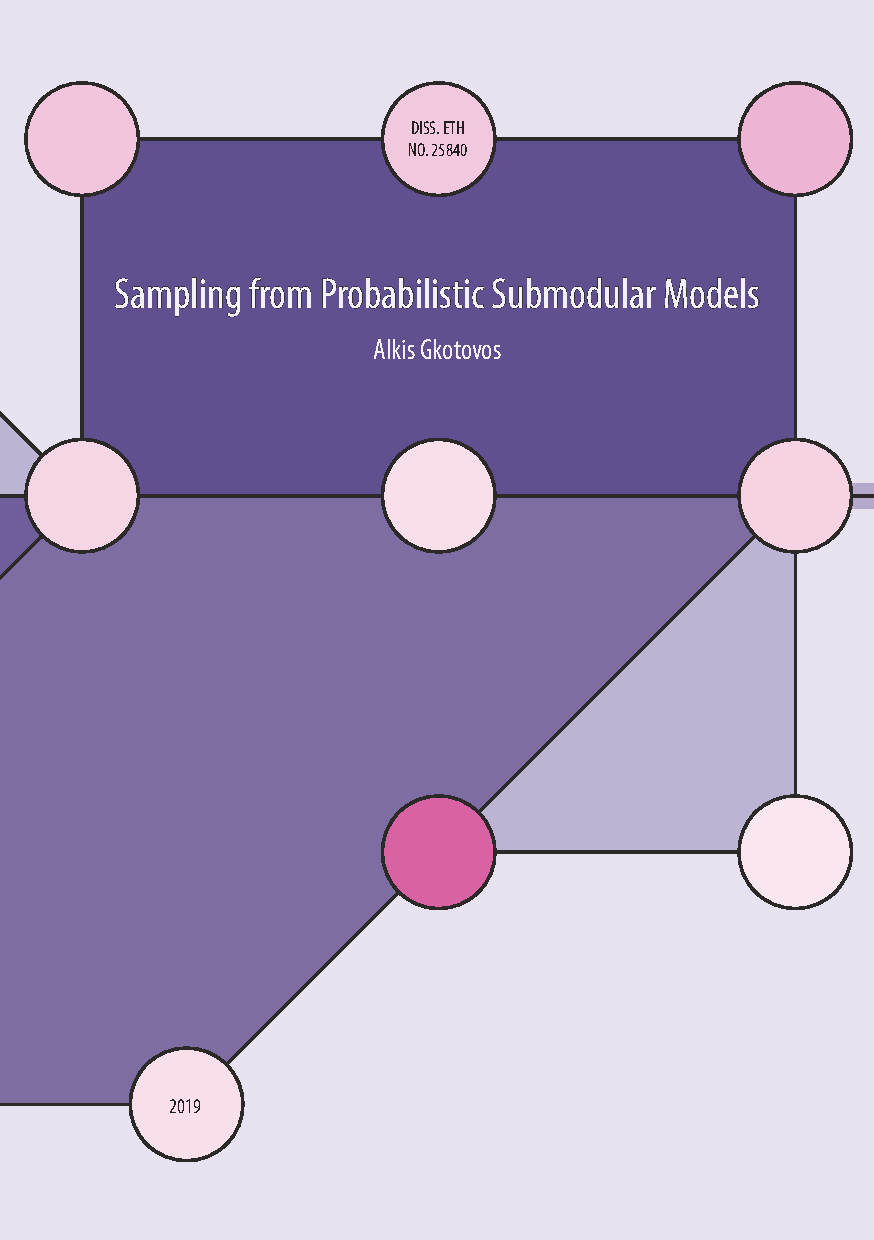
\includepdf[pages={1}]{title/outer.pdf}
\includepdf[pages={1}]{title/inner.pdf}

\cleardoublepage
\section*{\centering Abstract}
\vspace{1em}
Practical problems of discrete nature are very common in machine learning; application domains include computer vision (e.g., image segmentation), sequential decision making (e.g., active learning), social network analysis (e.g., influence maximization), and natural language processing (e.g., document summarization).
Submodular set functions have found wide applicability in such problems for their ability to capture notions of coverage, diversity, or exclusivity; analogously, supermodular set functions have been used to capture notions of regularity, smoothness, or co-occurrence.

While the topic of submodular optimization has received much attention, these functions can also be used to define expressive discrete probabilistic models, called probabilistic submodular models.
Going beyond optimization, these models allow us to quantify predictive uncertainty, and suggest a maximum likelihood approach for learning such functions from noisy data.
Prominent examples of probabilistic submodular models include Ising and Potts models, as well as determinantal point processes, but the general class is much richer and little studied.

It is well known, though, that performing probabilistic inference in such models is computationally intractable in general.
In this thesis, we investigate the use of Markov chain Monte Carlo sampling as a means of performing approximate inference in probabilistic submodular models.

We start with analyzing the Gibbs sampler, and establish theoretical conditions that guarantee efficient convergence of this sampler in probabilistic submodular models.
We next propose a novel sampling procedure that makes use of discrete semigradients to perform efficient global moves, so as to avoid so-called state-space bottlenecks, and thus lead to improved convergence behavior.
Finally, we employ the aforementioned sampling methods to approximate the likelihood gradients, and learn such models from data.
More specifically, we apply our learning procedure to the problem of modeling interactions between genetic mutations in cancer patients, and demonstrate considerable improvement over the state of the art in many of our experimental results on both synthetic and real cancer data.

\cleardoublepage
\section*{Zusammenfassung}

\cleardoublepage
\section*{Acknowledgements}
\todo{}
\tableofcontents

\mainmatter
\pagestyle{mainmatter}
\renewcommand{\chaptermark}[1]{\markboth{#1}{}}
%\renewcommand{\chaptermark}[1]{\markright{\thechapter #1}}

\chapter{Introduction} \label{ch:intro}
To introduce the main concepts of this thesis, we begin with a motivation application from the field of cancer genomics.
One of the major undertakings in large-scale cancer genomics research projects, such as The Cancer Genome Atlas \citep{tcga}, is obtaining and analyzing genetic data from cancer patients.
Beyond investigating the occurrence of genetic mutations one by one, it is of particular interest to discover meaningful interactions between groups of mutations.

For example, it has been observed that, depending on the type of cancer, there are groups of specific mutations that are approximately mutually exclusive, that is, most of the time no more than one mutation from a particular group occurs in the same patient \citep{yeang08}.
Biologically this is explained by the fact that so-called driver mutations, i.e., mutations that are crucial in cancer development, often occur in a limited number of biological pathways, and mutations that affect a specific pathway tend to not occur in the same patient.
Taking this in the opposite direction, discovering groups of mutually exclusive mutations may be helpful in uncovering the structure of cancer-related pathways, and identifying important groups of driver mutations.

More concretely, assume that we are given a data set of $n$ mutations and $m$ patients.
In the simplest case, the data set contains only binary information about whether or not each mutation $i \in [n]$ occurs in each patient $j \in [m]$.
Equivalently, this can be encoded using a binary matrix, as shown in \figref{fig:bamat_1}.

\begin{figure}[htb]
\centering
\includegraphics[width=0.9\textwidth]{figures/intro/example1.pdf}\\[1em]
\caption{An example binary mutation matrix, in which each shaded entry $(i, j)$ indicates that mutation $i$ occured in patient $j$.}
\label{fig:bamat_1}
\end{figure}

In \figref{fig:bamat_2} we show a permuted version of the previous matrix, which illustrates that the first four mutations are approximately mutually exclusive.
Searching for such groups in data sets containing hundreds or thousands of mutations is a combinatorially daunting task.
Crucially, the available data is quite limited---TCGA data sets range from a few hundred to a couple of thousand patients---, and contains significant noise introduced by the employed measurement and preprocessing procedures.

\begin{figure}[tb]
\centering
\includegraphics[width=0.9\textwidth]{figures/intro/example1_rep.pdf}\\[1em]
\caption{The binary mutation matrix of the previous figure with permuted rows and columns to illustrate the mutual exclusivity between the first four mutations.}
\label{fig:bamat_2}
\end{figure}

Many practical machine learning problems are of discrete nature, that is, like the problem described above, they consist in choosing a subset out of a set of finite elements.
Examples include sensor placement \citep{krause06}, active learning \citep{golovin11}, influence maximization \citep{kempe03}, image segmentation \citep{jegelka11}, and document summarization \citep{lin11}.
While discrete optimization methods have been successful in many of these applications, it is often advantageous to go beyond optimization, and consider discrete probabilistic models.

The probabilistic nature of such models offers a way to deal with noisy data, and provides a flexible framework to robustly answer queries pertaining to the problem at hand.
Rather than having a single optimum as the solution, we have a way to quantify our uncertainty about the most likely configurations, and make robust decisions based on computing various marginal and conditional probabilities of interest (e.g., given that element $A$ is present, what is the probability that elements $B$ and $C$ are also present).
In addition, the use of probabilistic models suggests a principled approach for learning the potentially complex interactions present in the data, namely maximizing the likelihood of the model parameters.
Finally, constraining ourselves to specific model classes allows us to incorporate prior assumptions about the problem structure, and alleviate the scarce data issue.

\section{Thesis Topic \& Contributions}
Past research on discrete probabilistic models has primarily focused on models defined by pairwise interactions, such as Markov random fields \cite{koller09}.
In many applications, however, it is of importance to directly capture higher-order dependencies between larger groups of variables.
For example, in our aforementioned application, being able to directly encode larger groups of mutually exclusive mutations provides a potentially sparser and easier to interpret representation, while at the same time allowing for a richer structure of interactions.

On the other hand, in the context of discrete optimization, there has been extensive research on submodular set functions.
Submodularity is a diminishing returns property that has been used to encode repulsiveness or diversity; it can, thus, be applied to model mutual exlusivity between mutations in our application.
Analogously, its counterpart, supermodularity, has been used to encode attractiveness or cooperation, and can be used to model co-occurence of mutations in our application.
Notably, there exist well-known efficient algorithms for both approximate submodular maximization, as well as submodular minimization.

Merging these two directions naturally leads us to consider \emph{probabilistic submodular models} \citep{djolonga14,gotovos15}, a class of discrete probabilistic models defined by submodular (or supermodular) functions.
More concretely, given a ground set $V = \{1,\ldots n\}$, a probabilistic submodular model is a distribution over subsets of $V$ of the form
\begin{align*}
p(S; \btheta) = \frac{1}{Z(\btheta)} \exp\left( F(S; \btheta) \right),
\end{align*}
for all $S \subseteq V$, where $F$ is a submodular or supermodular function parameterized by $\btheta$, and $Z(\btheta)$ is the normalizer of the distribution.
Distributions of this form generalize some well-studied model classes, such as Ising models, and determinantal point processes.

\paragraph{Thesis topic.} Both learning the parameters $\btheta$ from data, as well as quantifying uncertainty and making decisions with the learned distribution, boil down to the fundamental task of probabilistic inference, that is, computing marginal probabilities or the normalizer $Z$ in such distributions, a problem that is known to be computationally intractable in general.
The main topic of this thesis is to investigate the use of Markov chain Monte Carlo sampling as a means of performing approximate inference in probabilistic submodular models.

\newpage
\paragraph{Contributions.} The primary contributions of this thesis can be summarized as follows.
\begin{itemize}[leftmargin=3.5em]
\item[\textsf{Chapter 3}] We analyze the Gibbs sampler in probabilistic submodular models, and prove sufficient theoretical conditions for polynomial-time, and fast---$\mathcal{O}(n\log n)$---mixing.
\item[\textsf{Chapter 4}] We propose a novel sampler that makes use of discrete semigradients to perform efficient global moves in the state space to avoid bottlenecks, thus leading to improved mixing over the Gibbs sampler.
\item[\textsf{Chapter 5}] We use sampling to learn probabilistic submodular models via approximate likelihood maximization, and apply this procedure to the problem of modeling interactions between genetic mutations in cancer patients.
Many of our results demonstrate considerable improvement over the state of the art.
\end{itemize}

\paragraph{Collaborators.}
The topic of sampling from probabilistic submodular models was conceived by my advisor, Prof. Andreas Krause, who has also contributed to most parts of this thesis by providing invaluable input and feedback over the years.
Parts of the theoretical analysis in \chapref{ch:gibbs}, and \chapref{ch:m3} were done in collaboration with Prof. Hamed Hassani.
The work of \chapref{ch:m3} was done under the guidance of Prof. Stefanie Jegelka, who also contributed to the theoretical analysis of this chapter.
Finally, regarding the application of \chapref{ch:genes}, I have had fruitful discussions with Gideon Dresdner, Dr. Kjong Lehmann, and Prof. Gunnar Rätsch.
\chapter{Gibbs Sampling in PSMs} \label{ch:gibbs}
Modeling notions such as coverage, representativeness, or diversity is an important challenge in many machine learning problems.
These notions are well captured by submodular set functions.
Analogously, supermodular functions capture notions of smoothness, regularity, or cooperation. 
As a result, submodularity and supermodularity, akin to concavity and convexity, have found numerous applications in machine learning.
The majority of previous work has focused on optimizing such functions, including the development and analysis of algorithms for minimization \cite{fujishige05} and maximization \cite{nemhauser78,feige07}, as well as the investigation of practical applications, such as sensor placement \cite{krause06}, active learning \cite{golovin11}, influence maximization \cite{kempe03}, and document summarization \cite{lin11}.

Beyond optimization, though, it is of interest to consider probabilistic models defined via submodular functions, that is, distributions over finite sets (or, equivalently, binary random vectors) defined as $p(S) \propto \exp(\beta F(S)),$ where $F : 2^V \to \mathbb{R}$ is a submodular or supermodular function (equivalently, either $F$ or $-F$ is submodular), and $\beta \geq 0$ is a scaling parameter.
Finding most likely sets in such models captures classical submodular optimization.
However, going beyond point estimates, that is, performing general probabilistic (e.g., marginal) inference in them, allows us to quantify uncertainty given some observations, as well as learn such models from data.
Only few special cases belonging to this class of models have been extensively studied in the past; most notably, Ising models \cite{koller09}, which are log-supermodular in the usual case of attractive (ferromagnetic) potentials, or log-submodular under repulsive (anti-ferromagnetic) potentials, and determinantal point processes \cite{kulesza12}, which are log-submodular.

Recently, \citet{djolonga14} considered a more general treatment of such models, and proposed a variational approach for performing approximate probabilistic inference for them.
It is natural to ask to what degree the usual alternative to variational methods, namely Monte Carlo sampling, is applicable to these models, and how it performs in comparison.
To this end, in this paper we consider a simple Markov chain Monte Carlo (MCMC) algorithm on log-submodular and log-supermodular models, and provide a first analysis of its performance.
We present two theoretical conditions that respectively guarantee polynomial-time and fast ($\mathcal{O}(n \log n)$) mixing in such models, and experimentally compare against the variational approximations on three examples.

\section{Problem Setup} \label{sect:setup}
We start by considering set functions $F : 2^V \to \mathbb{R}$, where $V$ is a finite ground set of size $|V| = n$.
Without loss of generality, if not otherwise stated, we will hereafter assume that $V = [n] \defeq \{1, 2, \ldots,n\}$.
The marginal gain obtained by adding element $v \in V$ to set $S \subseteq V$ is defined as $F(v|S) \defeq F(S \cup \{v\}) - F(S)$.
Intuitively, submodularity expresses a notion of diminishing returns; that is, adding an element to a larger set provides less benefit than adding it to a smaller one.
More formally, $F$ is submodular if, for any $S \subseteq T \subseteq V$, and any $v \in V \setminus T$, it holds that $F(v|T) \leq F(v|S)$.
Supermodularity is defined analogously by reversing the sign of this inequality.
In particular, if a function $F$ is submodular, then the function $-F$ is supermodular.
If a function $m$ is both submodular and supermodular, then it is called modular, and may be written in the form $m(S) = c + \sum_{v \in S} m_v$, where $c \in \mathbb{R}$, and $m_v \in \mathbb{R}$, for all $v \in V$.

Our main focus in this paper are distributions over the powerset of $V$ of the form
\begin{align}\label{eq:pdef}
p(S) = \frac{\exp(\beta F(S))}{Z},
\end{align}
for all $S \subseteq V$, where $F$ is submodular or supermodular.
The scaling parameter $\beta$ is referred to as inverse temperature, and distributions of the above form are called log-submodular or log-supermodular respectively.
The constant denominator $Z \defeq Z(\beta) \defeq \sum_{S \subseteq V} \exp(\beta F(S))$ serves the purpose of normalizing the distribution and is called the partition function of $p$.
An alternative and equivalent way of defining distributions of the above form is via binary random vectors $X \in \{0, 1\}^n$.
If we define $V(X) \defeq \sdef{v \in V}{X_v = 1}$, it is easy to see that the distribution $p_X(X) \propto \exp(\beta F(V(X)))$ over binary vectors is isomorphic to the distribution over sets of \eqref{eq:pdef}.
With a slight abuse of notation, we will use $F(X)$ to denote $F(V(X))$, and use $p$ to refer to both distributions.

\paragraph{Example models}
The (ferromagnetic) Ising model is an example of a log-supermodular model.
In its simplest form, it is defined through an undirected graph $(V, E)$, and a set of pairwise potentials $\sigma_{v,w}(S) \defeq 4(\mathds{1}_{\{v \in S\}}-0.5)(\mathds{1}_{\{w \in S\}}-0.5)$.
Its distribution has the form $p(S) \propto \exp(\beta\sum_{\{v,w\} \in E} \sigma_{v,w}(S))$, and is log-supermodular, because $F(S) = \sum_{\{v,w\} \in E} \sigma_{v,w}(S)$ is supermodular. (Each $\sigma_{v,w}$ is supermodular, and supermodular functions are closed under addition.)

Determinantal point processes (DPPs) are examples of log-submodular models.
A DPP is defined via a positive semidefinite matrix $K \in \mathbb{R}^{n \times n}$, and has a distribution of the form $p(S) \propto \det(K_S)$, where $K_S$ denotes the square submatrix indexed by $S$.
Since $F(S) = \ln \det(K_S)$ is a submodular function, $p$ is log-submodular.
Another example of log-submodular models are those defined through facility location functions, which have the form $F(S) = \sum_{\ell \in [L]} \max_{v \in S}w_{v,\ell}$, where $w_{v,\ell} \geq 0$, and are submodular.
If $w_{v,\ell} \in \{0, 1\}$, then $F$ represents a set cover function.

Note that, both the facility location model and the Ising model use decomposable functions, that is, functions that can be written as a sum of simpler submodular (resp. supermodular) functions $F_{\ell}$:
\begin{align} \label{eq:fdec}
F(S) = \sum_{\ell \in [L]} F_{\ell}(S).
\end{align}

\paragraph{Marginal inference}
Our goal is to perform marginal inference for the distributions described above.
Concretely, for some fixed $A \subseteq B \subseteq V$, we would like to compute the probability of sets $S$ that contain all elements of $A$, but no elements outside of $B$, that is, $p(A \subseteq S \subseteq B)$.
More generally, we are interested in computing conditional probabilities of the form $p(A \subseteq S \subseteq B \mid C \subseteq S \subseteq D)$.
This computation can be reduced to computing unconditional marginals as follows.
For any $C \subseteq V$, define the contraction of $F$ on $C$, $F_C : 2^{V \setminus C} \to \mathbb{R}$, by $F_C(S) = F(S \cup C) - F(S)$, for all $S \subseteq V \setminus C$.
Also, for any $D \subseteq V$, define the restriction of $F$ to $D$, $F^D : 2^D \to \mathbb{R}$, by $F^D(S) = F(S)$, for all $S \subseteq D$.
If $F$ is submodular, then its contractions and restrictions are also submodular, and, thus, $(F_C)^D$ is submodular.
Finally, it is easy to see that $p(S \mid C \subseteq S \subseteq D) \propto \exp(\beta (F_C)^D(S))$.
In our experiments, we consider computing marginals of the form $p(v \in S \mid C \subseteq S \subseteq D)$, for some $v \in V$, which correspond to $A = \{v\}$, and $B = V$.

\section{Sampling and Mixing Times}
Performing exact inference in models defined by \eqref{eq:pdef} boils down to computing the partition function $Z$.
Unfortunately, this is generally a \#P-hard problem, which was shown to be the case even for Ising models by Jerrum and Sinclair \cite{jerrum93}.
However, they also proposed a sampling-based FPRAS for a class of ferromagnetic models, which gives us hope that it may be possible to efficiently perform approximate inference in more general models under suitable conditions.

MCMC sampling \cite{levin08} approaches are based on performing randomly selected local moves in a state space $\ss$ to approximately compute quantities of interest.
The visited states $(X_0, X_1,\ldots)$ form a Markov chain, which under mild conditions converges to a stationary distribution $\pi$.
Crucially, the probabilities of transitioning from one state to another are carefully chosen to ensure that the stationary distribution is identical to the distribution of interest.
In our case, the state space is the powerset of $V$ (equivalently, the space of all binary vectors of length $n$), and to approximate the marginal probabilities of $p$ we construct a chain over subsets of $V$ that has stationary distribution $p$.

\paragraph{The Gibbs sampler}
In this paper, we focus on one of the simplest and most commonly used chains, namely the Gibbs sampler, also known as the Glauber chain.
We denote by $P$ the transition matrix of the chain; each element $P(x, y)$ corresponds to the conditional probability of transitioning from state $x$ to state $y$, that is, $P(x, y) \defeq \P[X_{t+1} = y \mid X_{t} = x]$, for any $x, y \in \ss$, and any $t \geq 0$.
We also define an adjacency relation $x \sim y$ on the elements of the state space, which denotes that $x$ and $y$ differ by exactly one element.
It follows that each $x \in \ss$ has exactly $n$ neighbors.

\begin{algorithm}[tb]
	\caption{Gibbs sampler}
	\label{alg:gibbs}
	\small{
		\begin{algorithmic}[1]
			\REQUIRE Ground set $V$, distribution $p(S) \propto \exp(\beta F(S))$
			\LET{$X_0$}{random subset of $V$}
			\FOR{$t = 0$ \TO $N_{\mathrm{iter}}$}
			\LET{$v$}{$\mathrm{Unif}(V)$}
			\LET{$\Delta_F(v | X_t)$}{$F(X_t \cup \{v\}) - F(X_t \setminus \{v\})$}
			\LET{$p_{\mathrm{add}}$}{$\exp(\beta\Delta_F(v | X_t))/(1 + \exp(\beta\Delta_F(v | X_t)))$}
			\LET{$z$}{$\mathrm{Unif}([0,1])$}
			\LINEIFELSE{$z \leq p_{\mathrm{add}}$}{$X_{t+1} \gets X_t \cup \{v\}$}{$X_{t+1} \gets X_t \setminus \{v\}$}
			\ENDFOR
		\end{algorithmic}
	}
\end{algorithm}

The Gibbs sampler is defined by an iterative two-step procedure, as shown in \algoref{alg:gibbs}.
First, it selects an element $v \in V$ uniformly at random; then, it adds or removes $v$ to the current state $X_t$ according to the conditional probability of the resulting state.
Importantly, the conditional probabilities that need to be computed do not depend on the partition function $Z$, thus the chain can be simulated efficiently, even though $Z$ is unknown and hard to compute.
Moreover, it is easy to see that $\Delta_F(v | X_t) = \mathds{1}_{\{v\not\in X_t\}}F(v|X_t) + \mathds{1}_{\{v\in X_t\}}F(v|X_t\setminus\{v\})$; thus, the sampler only requires a black box for the marginal gains of $F$, which are often faster to compute than the values of $F$ itself.
Finally, it is easy to show that the stationary distribution of the chain constructed this way is $p$.

\paragraph{Mixing times}
Approximating quantities of interest using MCMC methods is based on using time averages to estimate expectations over the desired distribution.
In particular, we estimate the expected value of function $f : \ss \to \mathbb{R}$ by $\E_p[f(X)] \approx (1/T)\sum_{r=1}^{T} f(X_{s + r})$.
For example, to estimate the marginal $p(v \in S)$, for some $v \in V$, we would define $f(x) = \mathds{1}_{\{x_v = 1\}}$, for all $x \in \ss$.
The choice of burn-in time $s$ and number of samples $T$ in the above expression presents a tradeoff between computational efficiency and approximation accuracy.
It turns out that the effect of both $s$ and $T$ is largely dependent on a fundamental quantity of the chain called \emph{mixing time} \cite{levin08}.

The mixing time of a chain quantifies the number of iterations $t$ required for the distribution of $X_t$ to be close to the stationary distribution $\pi$.
More formally, it is defined as $\tme \defeq \min \sdef{t}{d(t) \leq \epsilon}$, where $d(t)$ denotes the worst-case (over the starting state $X_0$ of the chain) total variation distance between the distribution of $X_t$ and $\pi$.
Establishing upper bounds on the mixing time of our Gibbs sampler is, therefore, sufficient to guarantee efficient approximate marginal inference (e.g., see Theorem 12.19 of \citet{levin08}).

\section{Theoretical Results}
In the previous section we mentioned that exact computation of the partition function for the class of models we consider here is, in general, infeasible.
Only for very few exceptions, such as DPPs, is exact inference possible in polynomial time \cite{kulesza12}.
Even worse, it has been shown that the partition function of general Ising models is hard to approximate; in particular, there is no FPRAS for these models, unless RP = NP \cite{jerrum93}.
This implies that the mixing time of any Markov chain with such a stationary distribution will, in general, be exponential in $n$.
It is, therefore, our aim to derive sufficient conditions that guarantee sub-exponential mixing times for the general class of models.

In some of our results we will use the fact that any submodular function $F$ can be written as
\begin{align} \label{eq:decomp}
  F = c + m + f,
\end{align}
where $c \in \mathbb{R}$ is a constant that has no effect on distributions defined by \eqref{eq:pdef}; $m$ is a normalized ($m(\varnothing) = 0$) modular function; and $f$ is a normalized ($f(\varnothing) = 0$) monotone submodular function, that is, it additionally satisfies the monotonicity property $f(v|S) \geq 0$, for all $v \in V$, and all $S \subseteq V$.
A similar decomposition is possible for any supermodular function as well.

%To further highlight the hardness of inference in the general models we consider, we show that even for distributions defined through a seemingly benign subclass of submodular functions, mixing times can be exponential in $n$.
%We say that a set function $F : 2^V \to \mathbb{R}$ is monotone, if $F(v|S) \geq 0$, for all $v \in V$, and all $S \subseteq V$.
%Intuitively, adding elements to our set always leads to higher values.
%\begin{lemma}
%There is a family of monotone submodular functions $F_n$, such that, for the corresponding log-submodular family of distributions $p_n$ defined as in \eqref{eq:pdef}, the Metropolis chain has mixing time
%\begin{align*}
%  \tm  = \Omega(2^{n/2}),
%\end{align*}
%\end{lemma}
%for any value of $\beta$.
%
%The functions used to prove the above lemma are based on the following construction.
%For any even $n \geq 2$, let $V_n = \{1,\ldots,n\}$, $R_n = \{1,\ldots,n/2\}$, and $C_n = \{n/2+1,\ldots,n\}$.
%To define function $F_n : 2^{V_n} \to \mathbb{R}$, we conceptually use a $n/2 \times n/2$ square grid, whose rows are indexed by $R$ and columns by $C$.
%Each cell $(i, j)$ of the grid is considered to be covered if either row $i \in R$ or column $j \in C$ is selected.
%Formally, we define $F_n$ by
%\begin{align*}
%  F_n(S) = \frac{4}{n^2}\big\vert \sdef{(i, j) \in R \times C}{i \in S \lor j \in S}\big\vert,
%\end{align*}
%for any $S \subseteq V_n$, which results in $F_n(V_n) = 1$.
%
%Assume a Metropolis chain with transition matrix $P$, and stationary distribution $p_n(S) \propto \exp(\beta F_n(S))$.
%
%\newcommand{\subflen}{0.49\textwidth}
%\newcommand{\scspacey}{0em}
%\newcommand{\scspacex}{0em}
%\begin{figure}[tb]
%  \captionsetup[subfigure]{oneside,margin={2em,0em}}
%  \begin{subfigure}[b]{\subflen}
%	\centering
%	\begin{tikzpicture}[
%	%baseline,
%	scale=1
%	]
%	\fill[blue!40!white] (-2,1) rectangle (2,2);
%	\fill[blue!40!white] (-2,-1) rectangle (2,0);
%	\fill[blue!40!white] (0,-2) rectangle (1,2);
%	\draw[step=1cm,gray!80!black,line width=0.15em,line join=miter] (-2.01,-2.01) grid (2.01,2.01);
%	
%	\node at (-2.5,1.5) {\normalsize$1$};
%	\node at (-2.5,0.5) {\normalsize$2$};
%	\node at (-2.5,-0.5) {\normalsize$3$};
%	\node at (-2.5,-1.5) {\normalsize$4$};
%	\node at (-1.5,2.5) {\normalsize$5$};
%	\node at (-0.5,2.5) {\normalsize$6$};
%	\node at (0.5,2.5) {\normalsize$7$};
%	\node at (1.5,2.5) {\normalsize$8$};
%	\end{tikzpicture}
%	%\caption{}
%	\label{fig:grid}
%  \end{subfigure}
%  \begin{subfigure}[b]{\subflen}
%  	\centering
%    \trimbox{3em 6em 3em 6em}{
%  	\begin{tikzpicture}[
%  	%baseline,
%  	scale=1,
%    VN/.style={fill=white,draw=gray!80!black,circle,line width=0.15em,minimum size=1.5em},
%    LL/.style={draw=gray!80!black,line width=0.1em}
%    ]
%    %\clip (-6,-4) rectangle (-6, -4);
%    \draw [LL,fill=gray!30!white] (0,0) .. controls (4,4) and (4,-4) .. (0,0);
%    \draw [LL,fill=gray!30!white] (0,0) .. controls (-4,4) and (-4,-4) .. (0,0);
%    \node [VN] (V) at (0,0) {$V$};
%    \node (R) at (-1.8, 0) {$\mathcal{R}$};
%    \node (C) at (1.8, 0) {$\mathcal{C}$};
%  	\end{tikzpicture}}
%  	%\caption{}
%  	\label{fig:ss}
%  \end{subfigure}
%  \caption{\emph{Left.} Example grid for $n = 8$ with the cells corresponding to $F_8(\{1,3,7\})$ shown shaded. \emph{Right.} Illustration of the state space and the bottleneck at $V$.}
%\end{figure}
%
\subsection{Polynomial-time mixing} \label{sect:poly}
Our guarantee for mixing times that are polynomial in $n$ depends crucially on the following quantity, which is defined for any set function $F : 2^V \to \mathbb{R}$:
\begin{align*}
  \zf \defeq \max_{A, B \subseteq V} \left|F(A) + F(B) - F(A \cup B) - F(A \cap B) \right|.
\end{align*}
Intuitively, $\zf$ quantifies a notion of distance to modularity.
To see this, note that a function $F$ is modular if and only if $F(A) + F(B) = F(A \cup B) + F(A \cap B)$, for all $A, B \subseteq V$.
For modular functions, therefore, we have $\zf = 0$.
Furthermore, a function $F$ is submodular if and only if $F(A) + F(B) \geq F(A \cup B) + F(A \cap B)$, for all $A, B \subseteq V$.
Similarly, $F$ is supermodular if the above holds with the sign reversed.
It follows that for submodular and supermodular functions, $\zf$ represents the worst-case amount by which $F$ violates the modular equality.
It is also important to note that, for submodular and supermodular functions, $\zf$ depends only on the monotone part of $F$; if we decompose $F$ according to \eqref{eq:decomp}, then it is easy to see that $\zf = \zeta_f$.
A trivial upper bound on $\zf$, therefore, is $\zf \leq f(V)$.
Another quantity that has been used in the past to quantify the deviation of a submodular function from modularity is the curvature \cite{conforti84}, defined as $\kappa_F \defeq 1 - \min_{v \in V} \left(F(v|V\setminus\{v\}) / F(v)\right)$.
Although of similar intuitive meaning, the multiplicative nature of its definition makes it significantly different from $\zf$, which is defined additively.

As an example of a function class with $\zf$ that do not depend on $n$, assume a ground set $V = \bigcup_{\ell = 1}^L V_{\ell}$, and consider functions $F(S) = \sum_{\ell = 1}^L \phi(|S \cap V_{\ell}|)$, where $\phi : \mathbb{R} \to \mathbb{R}$ is a bounded concave function, for example, $\phi(x) = \min\{\phi_{\max}, x\}$.
Functions of this form are submodular, and have been used in applications such as document summarization to encourage diversity \cite{lin11}.
It is easy to see that, for such functions, $\zf \leq L\phi_{\max}$, that is, $\zf$ is independent of $n$.

The following theorem establishes a bound on the mixing time of the Gibbs sampler run on models of the form \eqref{eq:pdef}.
The bound is exponential in $\zf$, but polynomial in $n$.
\begin{theorem} \label{thm:poly}
  For any function $F : 2^V \to \mathbb{R}$, the mixing time of the Gibbs sampler is bounded by
  \begin{align*}
    \tme \leq 2n^2 \exp(2 \beta \zf) \log\left(\frac{1}{\epsilon p_{\min}}\right),
  \end{align*}
  where $p_{\min} \defeq \displaystyle\min_{S \in \ss}p(S)$.
  If $F$ is submodular or supermodular, then the bound is improved to
  \begin{align*}
    \tme \leq 2n^2 \exp(\beta \zeta_f) \log\left(\frac{1}{\epsilon p_{\min}}\right).
  \end{align*}
\end{theorem}
Note that, since the factor of two that constitutes the difference between the two statements of the theorem lies in the exponent, it can have a significant impact on the above bounds.
The dependence on $p_{\min}$ is related to the (worst-case) starting state of the chain, and can be eliminated if we have a way to guarantee a high-probability starting state.
If $F$ is submodular or supermodular, this is usually straightforward to accomplish by using one of the standard constant-factor optimization algorithms \cite{nemhauser78,fujishige05} as a preprocessing step.
More generally, if $F$ is bounded by $0 \leq F(S) \leq F_{\max}$, for all $S \subseteq V$, then $\log (1/p_{\min}) = \mathcal{O}(n \beta F_{\max})$.

\paragraph{Canonical paths}
Our proof of \theoremref{thm:poly} is based on the method of \emph{canonical paths} \cite{jerrum03,sinclair92,jerrum89,diaconis91}.
The high-level idea of this method is to view the state space as a graph, and try to construct a path between each pair of states that carries a certain amount of flow specified by the stationary distribution under consideration.
Depending on the choice of these paths and the resulting load on the edges of the graph, we can derive bounds on the mixing time of the Markov chain.

More concretely, let us assume that for some set function $F$ and corresponding distribution $p$ as in \eqref{eq:pdef}, we construct the Gibbs chain on state space $\ss = 2^V$ with transition matrix $P$.
We can view the state space as a directed graph that has vertex set $\ss$, and for any $A, B \in \ss$, contains edge $(S, S')$ if and only if $S \sim S'$, that is, if and only if $S$ and $S'$ differ by exactly one element.
Now, assume that, for any pair of states $A, B \in \ss$, we define what is called a canonical path $\gamma_{AB} \defeq (A = S_0, S_1, \ldots, S_{\ell} = B)$, such that all $(S_i, S_{i+1})$ are edges in the above graph.
We denote the length of path $\gamma_{AB}$ by $|\gamma_{AB}|$, and define $Q(S, S') \defeq p(S) P(S, S')$.
We also denote the set of all pairs of states whose canonical path goes through $(S, S')$ by $\mathcal{C}_{SS'} \defeq \sdef{(A, B) \in \ss \times \ss}{(S, S') \in \gamma_{AB}}$.
The following quantity, referred to as the \emph{congestion} of an edge, uses a collection of canonical paths to quantify to what amount that edge is overloaded:
\begin{align} \label{eq:cong}
  \rho(S, S') \defeq \frac{1}{Q(S, S')} \sum_{(A, B) \in \mathcal{C}_{SS'}} p(A) p(B) |\gamma_{AB}|.
\end{align}
The denominator $Q(S, S')$ quantifies the capacity of edge $(S, S')$, while the sum represents the total flow through that edge according to the choice of canonical paths.
The congestion of the whole graph is then defined as $\rho \defeq \max_{S \sim S'}\rho(S, S')$.
Low congestion implies that there are no bottlenecks in the state space, and the chain can move around fast, which also suggests rapid mixing.
The following theorem makes this concrete.

\begin{theorem}[\hspace{1sp}\cite{sinclair92,jerrum03}] \label{thm:cpath}
  For any collection of canonical paths with congestion $\rho$, the mixing time of the chain is bounded by
  \begin{align*}
  	\tme \leq \rho \log\left(\frac{1}{\epsilon p_{\mathrm{min}}}\right).
  \end{align*}
%  where $p_{\min} \defeq \displaystyle\min_{S \in \ss}p(S)$.
\end{theorem}

\paragraph{Proof outline of \theoremref{thm:poly}}
To apply \theoremref{thm:cpath} to our class of distributions, we need to construct a set of canonical paths in the corresponding state space $2^V$, and upper bound the resulting congestion.
First, note that, to transition from state $A \in \ss$ to state $B \in \ss$, in our case, it is enough to remove the elements of $A \setminus B$ and add the elements of $B \setminus A$.
Each removal and addition corresponds to an edge in the state space graph, and the order of these operations identify a canonical path in this graph that connects $A$ to $B$.
For our analysis, we assume a fixed order on $V$ (e.g., the natural order of the elements themselves), and perform the operations according to this order.

Having defined the set of canonical paths, we proceed to bounding the congestion $\rho(S, S')$ for any edge $(S, S')$.
The main difficulty in bounding $\rho(S, S')$ is due to the sum in \eqref{eq:cong} over all pairs in $\mathcal{C}_{SS'}$.
To simplify this sum we construct for each edge $(S, S')$ an injective map $\ess : \mathcal{C}_{SS'} \to \ss$; this is a combinatorial encoding technique that has been previously used in similar proofs to ours \cite{jerrum03}.
We then prove the following key lemma about these maps.

\begin{lemma} \label{lem:poly}
  For any $S \sim S'$, and any $A, B \in \ss$, it holds that
  \begin{align*}
  	p(A)p(B) \leq 2n\exp(2 \beta \zf)Q(S, S')p(\ess(A, B)).
  \end{align*}
\end{lemma}

Since $\ess$ is injective, it follows that $\sum_{(A, B) \in \mathcal{C}_{SS'}} p(\ess(A, B)) \leq 1$.
Furthermore, it is clear that each canonical path $\gamma_{AB}$ has length $|\gamma_{AB}| \leq n$, since we need to add and/or remove at most $n$ elements to get from state $A$ to state $B$.
Combining these two facts with the above lemma, we get
\begin{align*}
  \rho(S, S') \leq 2n^2 \exp(2 \beta \zf).
\end{align*}
If $F$ is submodular or supermodular, we show that the dependence on $\zf$ in \lemmaref{lem:poly}  is improved to $\exp(\beta \zf)$.
More details can be found in the longer version of the paper.

\subsection{Fast mixing}
We now proceed to show that, under some stronger conditions, we are able to establish even faster---$\mathcal{O}(n \log n)$---mixing.
For any function $F$, we denote $\D_F(v|S) \defeq F(S \cup \{v\}) - F(S \setminus \{v\})$, and define the following quantity,
\begin{align*}
  \gf &\defeq \max_{\substack{S \subseteq V\\r \in V}} \sum_{\substack{v \in V}} \tanh\left(\frac{\beta}{2} \big|\D_F(v|S) - \D_F(v|S \cup \{r\})\big| \right),
\end{align*}

which quantifies the (maximum) total influence of an element $r \in V$ on the values of $F$.
For example, if the inclusion of $r$ makes no difference with respect to other elements of the ground set, we will have $\gf = 0$.
The following theorem establishes conditions for fast mixing of the Gibbs sampler when run on models of the form \eqref{eq:pdef}.

\begin{theorem} \label{thm:fast}
  For any set function $F : 2^V \to \mathbb{R}$, if $\gf < 1$, then the mixing time of the Gibbs sampler is bounded by
  \begin{align*}
  	\tme \leq \frac{1}{1 - \gf}n(\log n + \log \frac{1}{\epsilon}).
  \end{align*}
  If $F$ is additionally submodular or supermodular, and is decomposed according to \eqref{eq:decomp}, then
  \begin{align*}
  	\tme \leq \frac{1}{1 - \gsf}n(\log n + \log \frac{1}{\epsilon}).
  \end{align*}
\end{theorem}
Note that, in the second part of the theorem, $\gsf$ depends only on the monotone part of $F$. 
We have seen in \sectref{sect:setup} that some commonly used models are based on decomposable functions that can be written in the form \eqref{eq:fdec}.
We prove the following corollary that provides an easy to check condition for fast mixing of the Gibbs sampler when $F$ is a decomposable submodular function.

\begin{cor} \label{cor:fast}
  For any submodular function $F$ that can be written in the form of \eqref{eq:fdec}, with $f$ being its monotone (also decomposable) part according to \eqref{eq:decomp}, if we define
  \begin{align*}
  	\theta_f \defeq \max_{v \in V} \sum_{\ell \in [L]} \sqrt{f_{\ell}(v)} \hspace{1em}\textrm{and}\hspace{1em} \lambda_f \defeq \max_{\ell \in [L]} \sum_{v \in V} \sqrt{f_{\ell}(v)},
  \end{align*}
  then it holds that
  \begin{align*}
  	\gsf \leq \frac{\beta}{2} \theta_f \lambda_f.
  \end{align*}
\end{cor}

For example, applying this to the facility location model defined in \sectref{sect:setup}, we get $\theta_f = \max_{v} \sum_{\ell = 1}^L \sqrt{w_{v, \ell}}$, and $\lambda_f = \max_{\ell} \sum_{v \in V} \sqrt{w_{v, \ell}}$, and obtain fast mixing if $\theta_f \lambda_f \leq 2/\beta$.
As a special case, if we consider the class of set cover functions ($w_{v, \ell} \in \{0, 1\}$), such that each $v \in V$ covers at most $\delta$ sets, and each set $\ell \in [L]$ is covered by at most $\delta$ elements, then $\theta_f, \lambda_f \leq \delta$, and we obtain fast mixing if $\delta^2 \leq 2/\beta$.
Note, that the corollary can be trivially applied to any submodular function by taking $L=1$, but may, in general, result in a loose bound if used that way.

\paragraph{Coupling}
Our proof of \theoremref{thm:fast} is based on the \emph{coupling} technique \cite{aldous83}; more specifically, we use the \emph{path coupling} method \cite{bubley97,levin08,jerrum03}.
Given a Markov chain $(X_t)$ on state space $\ss$ with transition matrix $P$, a coupling for $(Z_t)$ is a new Markov chain $(X_t, Y_t)$ on state space $\ss \times \ss$, such that both $(X_t)$ and $(Y_t)$ are by themselves Markov chains with transition matrix $P$.
The idea is to construct the coupling in such a way that, even when the starting points $X_0$ and $Y_0$ are different, the chains $(X_t)$ and $(Y_t)$ tend to coalesce.
Then, it can be shown that the coupling time $t_{\mathrm{couple}} \defeq \min\sdef{t \geq 0}{X_t = Y_t}$ is closely related to the mixing time of the original chain $(Z_t)$. \cite{levin08}

The main difficulty in applying the coupling approach lies in the construction of the coupling itself, for which one needs to consider any possible pair of states $(Y_t, Z_t)$.
The path coupling technique makes this construction easier by utilizing the same state-space graph that we used to define canonical paths in \sectref{sect:poly}.
The core idea is to first define a coupling only over adjacent states, and then extend it for any pair of states by using a metric on the graph.
More concretely, let us denote by $d : \ss \times \ss \to \mathbb{R}$ the \emph{path metric} on state space $\ss$; that is, for any $x, y \in \ss$, $d(x, y)$ is the minimum length of any path from $x$ to $y$ in the state space graph.
The following theorem establishes fast mixing using this metric, as well as the diameter of the state space, $\mathrm{diam}(\ss) \defeq \max_{x,y \in \ss}d(x, y)$.
\begin{theorem}[\hspace{1sp}\cite{bubley97,levin08}] \label{thm:pc}
For any Markov chain $(Z_t)$, if $(X_t, Y_t)$ is a coupling, such that, for some $a \geq 0$, and any $x, y \in \ss$ with $x \sim y$, it holds that
\begin{align*}
  \E[d(X_{t+1}, Y_{t+1}) \mid X_t = x, Y_t = y] \leq e^{-\alpha}d(x, y),
\end{align*}
then the mixing time of the original chain is bounded by
\begin{align*}
  \tme \leq \frac{1}{\alpha}\left(\log(\mathrm{diam}(\ss)) + \log\frac{1}{\epsilon} \right).
\end{align*}
\end{theorem}

\paragraph{Proof outline of \theoremref{thm:fast}}
In our case, the path metric $d$ is the Hamming distance between the binary vectors representing the states (equivalently, the number of elements by which two sets differ).
We need to construct a suitable coupling $(X_t, Y_t)$ for any pair of states $x \sim y$.
Consider the two corresponding sets $S, R \subseteq V$ that differ by exactly one element, and assume that $R = S \cup \{r\}$, for some $r \in V$. (The case $S = R \cup \{s\}$ for some $s \in V$ is completely analogous.)
Remember that the Gibbs sampler first chooses an element $v \in V$ uniformly at random, and then adds or removes it according to the conditional probabilities.
Our goal is to make the same updates happen to both $S$ and $R$ as frequently as possible.
As a first step, we couple the candidate element for update $v \in V$ to always be the same in both chains.
Then, we have to distinguish between the following cases.

If $v = r$, then the conditionals for both chains are identical, therefore we can couple both chains to add $r$ with probability $p_{\mathrm{add}} \defeq p(S \cup \{r\}) / (p(S) + p(S \cup \{r\}))$, which will result in new sets $S' = R' = S \cup \{r\}$, or remove $r$ with probability $1 - p_{\mathrm{add}}$, which will result in new sets $S' = R' = S$.
Either way, we will have $d(S', R') = 0$.
  
If $v \neq r$, we cannot always couple the updates of the chains, because the conditional probabilities of the updates are different.
In fact, we are forced to have different updates (one chain adding $v$, the other chain removing $v$) with probability equal to the difference of the corresponding conditionals, which we denote here by $p_{\mathrm{dif}}(v)$.
%  \begin{align*}
%  	p_{\mathrm{dif}}(v) \defeq \left|\frac{p(S \cup \{v\})}{p(S \cup \{v\}) + p(S \setminus \{v\})} - \frac{p(R \cup \{v\})}{p(R \cup \{v\}) + p(R \setminus \{v\})}\right|.
%  \end{align*}
If this is the case, we will have $d(S', R') = 2$, otherwise the chains will make the same update and will still differ only by element $r$, that is, $d(S', R') = 1$.
  
Putting together all the above, we get the following expected distance after one step:
\begin{align*}
  \E[d(S', R')] = 1 -\frac{1}{n} + \frac{1}{n}\sum_{v \neq r}p_{\mathrm{dif}}(v) \leq 1 - \frac{1}{n}(1 - \gf) \leq \exp\left(-\frac{1-\gf}{n}\right).
\end{align*}
Our result follows from applying \theoremref{thm:pc} with $\alpha = \gf/n$, noting that $\mathrm{diam}(\ss) = n$.

\section{Experiments}
We compare the Gibbs sampler against the variational approach proposed by Djolonga and Krause \cite{djolonga14} for performing inference in models of the form \eqref{eq:pdef}, and use the same three models as in their experiments.
We briefly review here the experimental setup and refer to their paper for more details.

The first is a (log-submodular) facility location model with an added modular term that penalizes the number of selected elements, that is, $p(S) \propto \exp(F(S)-2|S|)$, where $F$ is a submodular facility location function.
The model is constructed from randomly subsampling real data from a problem of sensor placement in a water distribution network \cite{krause08}.
In the experiments, we iteratively condition on random observations for each variable in the ground set.
The second is a (log-supermodular) pairwise Markov random field (MRF; a generalized Ising model with varying weights), constructed by first randomly sampling points from a 2-D two-cluster Gaussian mixture model, and then introducing a pairwise potential for each pair of points with exponentially-decreasing weight in the distance of the pair.
In the experiments, we iteratively condition on pairs of observations, one from each cluster.
The third is a (log-supermodular) higher-order MRF, which is constructed by first generating a random Watts-Strogatz graph, and then creating one higher-order potential per node, which contains that node and all of its neighbors in the graph.
The strength of the potentials is controlled by a parameter $\mu$, which is closely related to the curvature of the functions that define them.
In the experiments, we vary this parameter from $0$ (modular model) to $1$ (``strongly'' supermodular model).

For all three models, we constrain the size of the ground set to $n = 20$, so that we are able to compute, and compare against, the exact marginals.
Furthermore, we run multiple repetitions for each model to account for the randomness of the model instance, and the random initialization of the Gibbs sampler.
The marginals we compute are of the form $p(v \in S \mid C \subseteq S \subseteq D)$, for all $v \in V$.
We run the Gibbs sampler for $100$, $500$, and $2000$ iterations on each problem instance.
In compliance with recommended MCMC practice \cite{gelman11}, we discard the first half of the obtained samples as burn-in, and only use the second half for estimating the marginals.

\figref{fig:exp} compares the average absolute error of the approximate marginals with respect to the exact ones.
The averaging is performed over $v \in V$, and over the different repetitions of each experiment; errorbars depict two standard errors.
The two variational approximations are obtained from factorized distributions associated with modular lower and upper bounds respectively \cite{djolonga14}.
We notice a similar trend on all three models.
For the regimes that correspond to less ``peaked'' posterior distributions (small number of conditioned variables, small $\mu$), even $100$ Gibbs iterations outperform both variational approximations.
The latter gain an advantage when the posterior is concentrated around only a few states, which happens after having conditioned on almost all variables in the first two models, or for $\mu$ close to $1$ in the third model.

\setlength\figureheight{0.285\textwidth}
\setlength\figurewidth{0.4\textwidth}
\newcommand{\subflen}{0.33\textwidth}
\newcommand{\scspacey}{-1.55em}
\newcommand{\scspacex}{0em}
\begin{figure}[tb]
  \captionsetup[subfigure]{oneside,margin={2em,0em}}
  \begin{subfigure}[b]{\subflen}
    \centering
    \begin{tikzpicture}

\begin{axis}[%
tick label style={font=\tiny},
label style={font=\scriptsize},
legend style={font=\scriptsize},
view={0}{90},
width=\figurewidth,
height=\figureheight,
xmin=0, xmax=19,
xtick={0, 2, 4, 6, 8, 10, 12, 14, 16, 18},
xlabel={Number of conditioned elements},
xlabel shift=-0.3em,
ymin=0, ymax=0.15,
%ylabel={Mean absolute error},
ylabel shift=-0.3em,
tick label style={/pgf/number format/fixed},
major tick length=2pt,
axis lines*=left,
legend cell align=left,
clip=false,
legend style={at={(1.05,1.05)},draw=none,row sep=-0.35em}]

\addplot [
mark=*,
mark size=1.3pt,
mark options={solid},
color=orange!60!black,
densely dashed,
line width=1pt,
error bars/.cd,
error bar style={solid, line width=1pt},
y dir=both,
y explicit
]
coordinates{
(0,0.107112366513)+- (2*0.00282243732842,2*0.00282243732842)(1,0.102922727287)+- (2*0.00298300698246,2*0.00298300698246)(2,0.0989540227828)+- (2*0.00303553867607,2*0.00303553867607)(3,0.0933829762656)+- (2*0.0031887954654,2*0.0031887954654)(4,0.0884069245638)+- (2*0.00337880496923,2*0.00337880496923)(5,0.0830474851382)+- (2*0.00339501861505,2*0.00339501861505)(6,0.0775476811889)+- (2*0.00353394763276,2*0.00353394763276)(7,0.072385269695)+- (2*0.00380613101446,2*0.00380613101446)(8,0.0690821376507)+- (2*0.0038559982422,2*0.0038559982422)(9,0.065985132415)+- (2*0.00423482988602,2*0.00423482988602)(10,0.0568044604494)+- (2*0.00405291178904,2*0.00405291178904)(11,0.0491925976389)+- (2*0.00407966954557,2*0.00407966954557)(12,0.0419781500303)+- (2*0.00434479981779,2*0.00434479981779)(13,0.0354290127274)+- (2*0.00410883118785,2*0.00410883118785)(14,0.0255396708993)+- (2*0.00333079208498,2*0.00333079208498)(15,0.021219417454)+- (2*0.0034504548739,2*0.0034504548739)(16,0.014942265471)+- (2*0.00320834756581,2*0.00320834756581)(17,0.00853834955108)+- (2*0.00274088479292,2*0.00274088479292)(18,0.00226092205199)+- (2*0.00144656700754,2*0.00144656700754)(19,4.35762537165e-17)+- (2*1.25377498951e-17,2*1.25377498951e-17)
};
\addlegendentry{Var (upper)}

\addplot [
mark=*,
mark size=1.3pt,
mark options={solid},
color=green!60!black,
densely dashed,
line width=1pt,
error bars/.cd,
error bar style={solid, line width=1pt},
y dir=both,
y explicit
]
coordinates{
(0,0.0787440547093)+- (2*0.00298005197383,2*0.00298005197383)(1,0.0742436730701)+- (2*0.00300217288835,2*0.00300217288835)(2,0.0718495604506)+- (2*0.00300216884821,2*0.00300216884821)(3,0.0677111346104)+- (2*0.00295406374421,2*0.00295406374421)(4,0.0631260247356)+- (2*0.00311734469971,2*0.00311734469971)(5,0.0601601130807)+- (2*0.00325485666533,2*0.00325485666533)(6,0.0555257803471)+- (2*0.0031801160993,2*0.0031801160993)(7,0.0516901198864)+- (2*0.00318849306217,2*0.00318849306217)(8,0.048428101947)+- (2*0.0030393789569,2*0.0030393789569)(9,0.0458999042102)+- (2*0.0031872052514,2*0.0031872052514)(10,0.0405156780929)+- (2*0.0031714204449,2*0.0031714204449)(11,0.0364292133548)+- (2*0.00322356186706,2*0.00322356186706)(12,0.0322789974519)+- (2*0.00353817833988,2*0.00353817833988)(13,0.0274526157463)+- (2*0.00330213737196,2*0.00330213737196)(14,0.0205765371103)+- (2*0.00273419570942,2*0.00273419570942)(15,0.0164503607956)+- (2*0.00282431409588,2*0.00282431409588)(16,0.0107574971385)+- (2*0.00234170467672,2*0.00234170467672)(17,0.00665211260322)+- (2*0.00230003884272,2*0.00230003884272)(18,0.00224240965205)+- (2*0.00129450418703,2*0.00129450418703)(19,4.35762537165e-17)+- (2*1.25377498951e-17,2*1.25377498951e-17)
};
\addlegendentry{Var (lower)}

\addplot [
mark=*,
mark size=1.3pt,
color=cyan!80!black,
line width=1pt,
error bars/.cd,
error bar style={line width=1pt},
y dir=both,
y explicit
]
coordinates{
(0,0.0473630182958)+- (2*0.000961855004575,2*0.000961855004575)(1,0.0481456982827)+- (2*0.00122148289021,2*0.00122148289021)(2,0.0486753310402)+- (2*0.00122350183561,2*0.00122350183561)(3,0.0487629521073)+- (2*0.00124401962589,2*0.00124401962589)(4,0.047527668065)+- (2*0.00117900106126,2*0.00117900106126)(5,0.0459422321573)+- (2*0.00126203739171,2*0.00126203739171)(6,0.0474112079185)+- (2*0.00132737883776,2*0.00132737883776)(7,0.0472267406495)+- (2*0.00154139765745,2*0.00154139765745)(8,0.0487267195556)+- (2*0.00166276183169,2*0.00166276183169)(9,0.0448581748084)+- (2*0.00162537810892,2*0.00162537810892)(10,0.0428964610789)+- (2*0.00158453345804,2*0.00158453345804)(11,0.0431304210258)+- (2*0.00154749821186,2*0.00154749821186)(12,0.0444676918443)+- (2*0.00146990599959,2*0.00146990599959)(13,0.0475667187549)+- (2*0.00174051373299,2*0.00174051373299)(14,0.038155307611)+- (2*0.00134271394952,2*0.00134271394952)(15,0.0396840457492)+- (2*0.00168491377663,2*0.00168491377663)(16,0.035141617162)+- (2*0.00188200219359,2*0.00188200219359)(17,0.0359254127362)+- (2*0.00171413997695,2*0.00171413997695)(18,0.0371142922613)+- (2*0.00213057040678,2*0.00213057040678)(19,0.0460605294728)+- (2*0.00336677118906,2*0.00336677118906)
};
\addlegendentry{Gibbs (100)}

\addplot [
mark=*,
mark size=1.3pt,
color=cyan!60!black,
line width=1pt,
error bars/.cd,
error bar style={line width=1pt},
y dir=both,
y explicit
]
coordinates{
(0,0.0218250134495)+- (2*0.000537303190621,2*0.000537303190621)(1,0.0224028180845)+- (2*0.000525654785107,2*0.000525654785107)(2,0.0219206177663)+- (2*0.000565826747106,2*0.000565826747106)(3,0.02104990332)+- (2*0.000573283890384,2*0.000573283890384)(4,0.0219281287808)+- (2*0.000595235228682,2*0.000595235228682)(5,0.0203873457403)+- (2*0.000594092511542,2*0.000594092511542)(6,0.0214753607454)+- (2*0.000660469200703,2*0.000660469200703)(7,0.0206945915246)+- (2*0.000625060240404,2*0.000625060240404)(8,0.0209477084508)+- (2*0.000687772701747,2*0.000687772701747)(9,0.0213575534533)+- (2*0.000714246634866,2*0.000714246634866)(10,0.020729536627)+- (2*0.000644018387617,2*0.000644018387617)(11,0.0193497488206)+- (2*0.000709749943125,2*0.000709749943125)(12,0.018856462422)+- (2*0.000765616207597,2*0.000765616207597)(13,0.019968403055)+- (2*0.00071527161823,2*0.00071527161823)(14,0.0182034664069)+- (2*0.000650300781802,2*0.000650300781802)(15,0.0187890961265)+- (2*0.00074087420748,2*0.00074087420748)(16,0.0184461841847)+- (2*0.000840727729976,2*0.000840727729976)(17,0.0189716928733)+- (2*0.000908520821074,2*0.000908520821074)(18,0.0185185555147)+- (2*0.00103564165586,2*0.00103564165586)(19,0.0204001588626)+- (2*0.00159590329676,2*0.00159590329676)
};
\addlegendentry{Gibbs (500)}

\addplot [
mark=*,
mark size=1.3pt,
color=cyan!40!black,
line width=1pt,
error bars/.cd,
error bar style={line width=1pt},
y dir=both,
y explicit
]
coordinates{
(0,0.0115035637873)+- (2*0.000253816939671,2*0.000253816939671)(1,0.0112576161002)+- (2*0.000286995311855,2*0.000286995311855)(2,0.0106906370982)+- (2*0.000248190003897,2*0.000248190003897)(3,0.0106140826962)+- (2*0.000338894626227,2*0.000338894626227)(4,0.0109692167346)+- (2*0.000274918741482,2*0.000274918741482)(5,0.0103752885383)+- (2*0.000282674963816,2*0.000282674963816)(6,0.0100551082539)+- (2*0.000270844679925,2*0.000270844679925)(7,0.0111432554282)+- (2*0.000371583391889,2*0.000371583391889)(8,0.00992150715657)+- (2*0.000301730849106,2*0.000301730849106)(9,0.0100765947272)+- (2*0.00033596761799,2*0.00033596761799)(10,0.0100544944077)+- (2*0.000274241462836,2*0.000274241462836)(11,0.00996175315692)+- (2*0.000334215423234,2*0.000334215423234)(12,0.0102649909643)+- (2*0.000407728757884,2*0.000407728757884)(13,0.00965189863135)+- (2*0.00035336738322,2*0.00035336738322)(14,0.00853533320694)+- (2*0.000295543887904,2*0.000295543887904)(15,0.00889231734521)+- (2*0.000501350216283,2*0.000501350216283)(16,0.00945549496442)+- (2*0.000376854406952,2*0.000376854406952)(17,0.00863467667401)+- (2*0.00039135687598,2*0.00039135687598)(18,0.00885232676003)+- (2*0.000484685835632,2*0.000484685835632)(19,0.00964430343626)+- (2*0.000741879337941,2*0.000741879337941)
};
\addlegendentry{Gibbs (2000)}

\end{axis}
\end{tikzpicture}
    \vspace{\scspacey}
    \caption{\hspace{\scspacex}Facility location}
    \label{fig:exp1}
  \end{subfigure}
  \begin{subfigure}[b]{\subflen}
    \begin{tikzpicture}

\begin{axis}[%
tick label style={/pgf/number format/fixed,font=\sffamily\small},
label style={font=\sffamily\small},
legend style={font=\sffamily\small},
view={0}{90},
width=\figurewidth,
height=\figureheight,
xmin=0, xmax=9,
xtick={0, 1, 2, 3, 4, 5, 6, 7, 8, 9},
xticklabels={0, 1, 2, 3, 4, 5, 6, 7, 8, 9},
xlabel={Number of conditioned pairs},
xlabel shift=0em,
ytick={0, 0.1, 0.2, 0.3, 0.4},
yticklabels={0, 0.1, 0.2, 0.3, 0.4},
ymin=0, ymax=0.4,
ylabel={Abs. marginal error},
ylabel shift=0em,
tick label style={/pgf/number format/fixed,font=\sffamily},
major tick length=2pt,
axis lines*=left,
legend cell align=left,
clip=false,
legend style={anchor=east,at={(1.4,0.5)},draw=none,row sep=0},
every axis plot/.append style={
  mark=*,
  mark options={solid},
  mark size=1.7pt,
  line width=1.2pt,
  opacity=0.9,
}
]

\addplot [
color=col2,
densely dashed,
error bars/.cd,
error bar style={solid, line width=1pt},
y dir=both,
y explicit
]
coordinates{
(0,0.00000)+-(0.00000,0.00000)(1,0.13529)+-(0.00946,0.00946)(2,0.15721)+-(0.00700,0.00700)(3,0.13708)+-(0.00529,0.00529)(4,0.10985)+-(0.00407,0.00407)(5,0.08099)+-(0.00343,0.00343)(6,0.05466)+-(0.00307,0.00307)(7,0.03219)+-(0.00203,0.00203)(8,0.01434)+-(0.00163,0.00163)(9,0.00002)+-(0.00001,0.00001)

};
\addlegendentry{Var (upper)}

\addplot [
color=col3,
densely dashed,
error bars/.cd,
error bar style={solid, line width=1pt},
y dir=both,
y explicit
]
coordinates{
(0,0.37813)+-(0.00543,0.00543)(1,0.18469)+-(0.00939,0.00939)(2,0.10135)+-(0.00621,0.00621)(3,0.06615)+-(0.00459,0.00459)(4,0.04468)+-(0.00314,0.00314)(5,0.03022)+-(0.00218,0.00218)(6,0.01988)+-(0.00164,0.00164)(7,0.01247)+-(0.00134,0.00134)(8,0.00556)+-(0.00096,0.00096)(9,0.00004)+-(0.00002,0.00002)

};
\addlegendentry{Var (lower)}

\addplot [
color=col1,
error bars/.cd,
error bar style={line width=1pt},
y dir=both,
y explicit
]
coordinates{
(0,0.33633)+-(0.01046,0.01046)(1,0.26388)+-(0.01602,0.01602)(2,0.20123)+-(0.01784,0.01784)(3,0.15406)+-(0.00906,0.00906)(4,0.13772)+-(0.00710,0.00710)(5,0.10925)+-(0.00641,0.00641)(6,0.10391)+-(0.00728,0.00728)(7,0.08370)+-(0.00673,0.00673)(8,0.06571)+-(0.00576,0.00576)(9,0.04372)+-(0.00535,0.00535)

};
\addlegendentry{Gibbs (200)}

\addplot [
color=col1!70!black,
error bars/.cd,
error bar style={line width=1pt},
y dir=both,
y explicit
]
coordinates{
(0,0.21841)+-(0.01672,0.01672)(1,0.14267)+-(0.01358,0.01358)(2,0.09997)+-(0.00997,0.00997)(3,0.07768)+-(0.00569,0.00569)(4,0.06026)+-(0.00361,0.00361)(5,0.05201)+-(0.00301,0.00301)(6,0.04489)+-(0.00266,0.00266)(7,0.03743)+-(0.00248,0.00248)(8,0.02995)+-(0.00245,0.00245)(9,0.01929)+-(0.00241,0.00241)

};
\addlegendentry{Gibbs (1000)}

\addplot [
color=col1!40!black,
error bars/.cd,
error bar style={line width=1pt},
y dir=both,
y explicit
]
coordinates{
(0,0.11321)+-(0.01234,0.01234)(1,0.07095)+-(0.00618,0.00618)(2,0.04435)+-(0.00305,0.00305)(3,0.03288)+-(0.00182,0.00182)(4,0.02745)+-(0.00137,0.00137)(5,0.02488)+-(0.00146,0.00146)(6,0.02025)+-(0.00146,0.00146)(7,0.01715)+-(0.00121,0.00121)(8,0.01316)+-(0.00107,0.00107)(9,0.00884)+-(0.00088,0.00088)

};
\addlegendentry{Gibbs (5000)}

\end{axis}
\end{tikzpicture}
    \vspace{\scspacey}
    \caption{\hspace{\scspacex}Pairwise MRF}
    \label{fig:exp2}
  \end{subfigure}
  \begin{subfigure}[b]{\subflen}
    \begin{tikzpicture}

\begin{axis}[%
tick label style={/pgf/number format/fixed,font=\sffamily\small},
label style={font=\sffamily\small},
legend style={font=\sffamily\small},
view={0}{90},
width=\figurewidth,
height=\figureheight,
xmin=0, xmax=1,
xtick={0, 0.2, 0.4, 0.6, 0.8, 1},
xticklabels={0, 0.2, 0.4, 0.6, 0.8, 1},
xlabel={$\mu$},
xlabel shift=0em,
ymin=0, ymax=0.15,
ytick={0, 0.05, 0.1, 0.15},
yticklabels={0, 0.05, 0.1, 0.15},
ylabel={Abs. marginal error},
ylabel shift=0em,
major tick length=2pt,
axis lines*=left,
legend cell align=left,
clip=false,
legend style={anchor=east,at={(1.4,0.5)},draw=none,row sep=0},
every axis plot/.append style={
  mark=*,
  mark options={solid},
  mark size=1.7pt,
  line width=1.2pt,
  opacity=0.9,
}
]

\addplot [
color=gcol2,
densely dashed,
error bars/.cd,
error bar style={solid, line width=1pt},
y dir=both,
y explicit
]
coordinates{
(0.01,0.07265)+-(0.00221,0.00221)(0.1189,0.06349)+-(0.00165,0.00165)(0.2278,0.05363)+-(0.00108,0.00108)(0.3367,0.04434)+-(0.00060,0.00060)(0.4456,0.03578)+-(0.00055,0.00055)((0.5544,0.02734)+-(0.00053,0.00053)(0.6633,0.02009)+-(0.00046,0.00046)(0.7722,0.01307)+-(0.00034,0.00034)(0.8811,0.00630)+-(0.00017,0.00017)(0.99,0.00050)+-(0.00002,0.00002)

};
\addlegendentry{Var (upper)}

\addplot [
color=gcol3,
densely dashed,
error bars/.cd,
error bar style={solid, line width=1pt},
y dir=both,
y explicit
]
coordinates{
(0.01,0.04309)+-(0.00738,0.00738)(0.1189,0.04162)+-(0.00706,0.00706)(0.2278,0.03337)+-(0.00505,0.00505)(0.3367,0.03534)+-(0.00472,0.00472)(0.4456,0.02535)+-(0.00388,0.00388)(0.5544,0.02088)+-(0.00247,0.00247)(0.6633,0.01532)+-(0.00153,0.00153)(0.7722,0.01047)+-(0.00126,0.00126)(0.8811,0.00547)+-(0.00054,0.00054)(0.99,0.00044)+-(0.00004,0.00004)

};
\addlegendentry{Var (lower)}

\addplot [
color=gcol1!50!white,
error bars/.cd,
error bar style={line width=1pt},
y dir=both,
y explicit
]
coordinates{
(0.01,0.08946)+-(0.01131,0.01131)(0.1189,0.09087)+-(0.00957,0.00957)(0.2278,0.09140)+-(0.00838,0.00838)(0.3367,0.09382)+-(0.00739,0.00739)(0.4456,0.09379)+-(0.00741,0.00741)(0.5544,0.10270)+-(0.00759,0.00759)(0.6633,0.11009)+-(0.00709,0.00709)(0.7722,0.10570)+-(0.00735,0.00735)(0.8811,0.10047)+-(0.00579,0.00579)(0.99,0.11209)+-(0.00756,0.00756)

};
\addlegendentry{Gibbs (200)}

\addplot [
color=gcol1,
error bars/.cd,
error bar style={line width=1pt},
y dir=both,
y explicit
]
coordinates{
(0.01,0.04593)+-(0.00491,0.00491)(0.1189,0.04659)+-(0.00466,0.00466)(0.2278,0.04902)+-(0.00465,0.00465)(0.3367,0.05229)+-(0.00452,0.00452)(0.4456,0.05153)+-(0.00349,0.00349)(0.5544,0.05246)+-(0.00351,0.00351)(0.6633,0.05408)+-(0.00386,0.00386)(0.7722,0.05374)+-(0.00316,0.00316)(0.8811,0.05628)+-(0.00312,0.00312)(0.99,0.05585)+-(0.00313,0.00313)

};
\addlegendentry{Gibbs (1000)}

\addplot [
color=gcol1!50!black,
error bars/.cd,
error bar style={line width=1pt},
y dir=both,
y explicit
]
coordinates{
(0.01,0.02303)+-(0.00238,0.00238)(0.1189,0.02210)+-(0.00170,0.00170)(0.2278,0.02145)+-(0.00192,0.00192)(0.3367,0.02355)+-(0.00190,0.00190)(0.4456,0.02305)+-(0.00171,0.00171)(0.5544,0.02423)+-(0.00148,0.00148)(0.6633,0.02533)+-(0.00155,0.00155)(0.7722,0.02373)+-(0.00120,0.00120)(0.8811,0.02506)+-(0.00162,0.00162)(0.99,0.02563)+-(0.00157,0.00157)

};
\addlegendentry{Gibbs (5000)}

\end{axis}
\end{tikzpicture}
    \vspace{\scspacey}
    \caption{\hspace{\scspacex}Higher-order MRF}
    \label{fig:exp3}
  \end{subfigure}
  \caption{Absolute error of the marginals computed by the Gibbs sampler compared to variational inference \cite{djolonga14}.
  	A modest $500$ Gibbs iterations outperform the variational method for the most part.}
  \label{fig:exp}
\end{figure}

\section{Further Related Work}
In contemporary work to ours, Rebeschini and Karbasi \cite{rebeschini15} analyzed the mixing times of log-submodular models.
Using a method based on matrix norms, which was previously introduced by Dyer et al. \cite{dyer09}, and is closely related to path coupling, they arrive at a similar---though not directly comparable---condition to the one we presented in \theoremref{thm:fast}.

Iyer and Bilmes \cite{iyer15} recently considered a different class of probabilistic models, called submodular point processes, which are also defined through submodular functions, and have the form $p(S) \propto F(S)$.
They showed that inference in SPPs is, in general, also a hard problem, and provided approximations and closed-form solutions for some subclasses.

The canonical path method for bounding mixing times has been previously used in applications, such as approximating the partition function of ferromagnetic Ising models \cite{jerrum93}, approximating matrix permanents \cite{jerrum89,jerrum04perm}, and counting matchings in graphs \cite{jerrum03}.
The most prominent application of coupling-based methods is counting $k$-colorings in low-degree graphs \cite{jerrum95,bubley98,jerrum03}.
Other applications include counting independent sets in graphs \cite{dyer00}, and approximating the partition function of various subclasses of Ising models at high temperatures \cite{levin08}.

\section{Conclusion}
We considered the problem of performing marginal inference using MCMC sampling techniques in probabilistic models defined through submodular functions.
In particular, we presented for the first time sufficient conditions to obtain upper bounds on the mixing time of the Gibbs sampler in general log-submodular and log-supermodular models.
Furthermore, we demonstrated that, in practice, the Gibbs sampler compares favorably to previously proposed variational approximations, at least in regimes of high uncertainty.
We believe that this is an important step towards a unified framework for further analysis and practical application of this rich class of probabilistic submodular models.
\appendix
\chapter{Detailed proofs}

\section{Polynomial-time Mixing Proofs}
For sets $A, B$, we denote $A \oplus B \defeq (A \setminus B)\cup(B \setminus A)$.

\let\oldthelemma\thelemma
\renewcommand{\thelemma}{A.1}
\begin{lemma} \label{lem:inj}
Define the maps $\ess : \mathcal{C}_{SS'} \to \ss$, for each pair $(S, S') \in \ss \times \ss$ with $S \sim S'$, as follows:
\begin{align*}
  \ess(A, B) = \twopartdefo{A \oplus B \oplus S}{F(S') \geq F(S)}{A \oplus B \oplus S'}.
\end{align*}
Then, each map $\ess$ is injective.
\end{lemma}

\begin{proof}
  Assume that $F(S') \geq F(S)$, and $S' = S \cup \{r\}$, for some $r \in V$.
  Assume that we are given $C \defeq A \oplus B \oplus S$, and we want to recover $A$ and $B$.
  We will denote by $\prec$ the natural ordering of the ground set $V$.
  First, we define
  \begin{align*}
    K^- &\defeq \sdef{v \in C \oplus S}{v \prec r}\\
    K^+ &\defeq \sdef{v \in C \oplus S}{v \succ r}.
  \end{align*}
  Then, we can recover $A$ and $V$ as follows:
  \begin{align*}
    A &= S \oplus K^-\\
    B &= S' \oplus K^+.
  \end{align*}
  The case $S' = S \setminus \{r\}$, as well as the two cases for $F(S') < F(S)$ are completely analogous.
  Note that the distinction based on the value of the function has no effect on the proof here, but is technically needed for the next lemma.
  The only thing that changes between the cases is whether the element $r$ that gets added or removed in the transition $(S, S')$ belongs to $A$ or $B$, which is always straightforward to determine from the type of the transition (for additions it belongs to $B$, and for removals to $A$).
\end{proof}
\let\thelemma\oldthelemma

\setcounter{lemma}{0}
\begin{lemma} \label{lem:poly_full}
  For any $S \sim S'$, and any $A, B \in \ss$, it holds that
  \begin{align*}
    p(A)p(B) \leq 2n\exp(2 \beta \zf)Q(S, S')p(\ess(A, B)).
  \end{align*}
  
  If $F$ is submodular or supermodular, then the bound is improved to
  \begin{align*}
  	p(A)p(B) \leq 2n\exp(\beta \zeta_f)Q(S, S')p(\ess(A, B)).
  \end{align*}
\end{lemma}

\begin{proof}
  We will consider the case $S' = S \cup \{r\}$, for some $r \in V$, with $F(S') \geq F(S)$.
  Again, the other three cases are completely analogous by using $\ess$ as defined in \lemmaref{lem:inj}.
  
  We first compute
  \begin{align*}
    Q(S, S') &= p(S)P(S, S')\\
             &= \frac{1}{n}\frac{p(S)p(S')}{p(S) + p(S')} \tag*{by definition of the Gibbs sampler}\\
             &= \frac{1}{nZ}\frac{\exp(\beta F(S)) \exp(\beta F(S'))}{\exp(\beta F(S)) + \exp(\beta F(S'))} \tag*{by definition of our models}\\
             &\geq \frac{1}{nZ}\frac{\exp(\beta F(S)) \exp(\beta F(S'))}{2\exp(\beta F(S'))} \tag*{by $F(S') \geq F(S)$}\\
             &= \frac{\exp(\beta F(S))}{2nZ}.
  \end{align*}
  As a result, we get
  \begin{align} \label{eq:ppq}
    \frac{p(A)p(B)}{Q(S, S')} \leq \frac{2n}{Z}\exp(\beta (F(A) + F(B) - F(S))).
  \end{align}
  Let us denote $\zf(A, B) \defeq F(A) + F(B) - F(A \cup B) - F(A \cap B)$, for any $A, B \subseteq V$, so that $\zf = \max_{A, B \subseteq V}|\zf(A, B)|$.
  Then, if we denote $C \defeq \ess(A, B) = A \oplus B \oplus S$, we have
  \begin{align*}
    &F(A) + F(B) - F(S)\\
    &= (F(A) + F(B) - F(A \cup B) - F(A \cap B)) - (F(S) + F(C) - F(A \cup B) - F(A \cap B)) + F(C)\\
    &= (F(A) + F(B) - F(A \cup B) - F(A \cap B)) - (F(S) + F(C) - F(S \cup C) - F(S \cap C)) + F(C)\\
    &= \zf(A, B) - \zf(S, C) + F(C)\\
    &\leq 2\zf + F(C).
  \end{align*}
  If $F$ is submodular, then $\zf(A, B)$ and $\zf(S, C)$ are both non-negative, therefore $\zf(A, B) - \zf(S, C) + F(C) \leq \zf + F(C) = \zeta_f + F(C)$.
  Similarly, if $F$ is supermodular, then $\zf(A, B)$ and $\zf(S, C)$ are both non-positive, therefore $\zf(A, B) - \zf(S, C) + F(C) \leq \zf + F(C) = \zeta_f + F(C)$.
  Substituting these bounds in \eqref{eq:ppq} gives us the result of the lemma.
\end{proof}

\section{Fast Mixing Proofs}

\let\oldthelemma\thelemma
\renewcommand{\thelemma}{B.1}
\begin{lemma}
For any $S, R \subseteq V$ with $R = S \cup \{r\}$, if we define
\begin{align*}
  p_{\mathrm{dif}}(v) \defeq \left|\frac{p(S \cup \{v\})}{p(S \cup \{v\}) + p(S \setminus \{v\})} - \frac{p(R \cup \{v\})}{p(R \cup \{v\}) + p(R \setminus \{v\})}\right|,
\end{align*}
then it holds that
\begin{align*}
  \sum_{v \neq r}p_{\mathrm{dif}}(v) \leq \gf.
\end{align*}
\end{lemma}
\let\thelemma\oldthelemma

\begin{proof}
  For any $v \neq r$, we have
  \begin{align*}
    p_{\mathrm{dif}}(v) &= \left|\frac{\exp(\beta F(S \cup \{v\}))}{\exp(\beta F(S \cup \{v\})) + \exp(\beta F(S \setminus \{v\}))} - \frac{\exp(\beta F(R \cup \{v\}))}{\exp(\beta F(R \cup \{v\})) + \exp(\beta F(R \setminus \{v\}))}\right|\\
    &= \left|\frac{\exp(\beta \D_F(v|S))}{1 + \exp(\beta \D_F(v|S))} - \frac{\exp(\beta \D_F(v|R))}{1 + \exp(\beta \D_F(v|R))}\right|\\
    &= \left|\frac{\exp(\beta \D_F(v|S)) - \exp(\beta \D_F(v|R))}{(1 + \exp(\beta \D_F(v|S)))(1 + \exp(\beta \D_F(v|R)))}\right|\\
    &\leq \left|\frac{\exp(\beta \D_F(v|S)) - \exp(\beta \D_F(v|R))}{\exp(\beta \D_F(v|S)) + \exp(\beta \D_F(v|R))}\right|\\
    &= \left|\frac{\exp(\beta (\D_F(v|S) - \D_F(v|R))) - 1}{\exp(\beta (\D_F(v|S) - \D_F(v|R))) + 1}\right|\\
    &= \tanh \left(\frac{\beta}{2}\big|(\D_F(v|S) - \D_F(v|R)) \big|\right).
  \end{align*}
  The lemma follows then by the definition of $\gf$, and the fact that $R = S \cup \{r\}$.
\end{proof}

\let\oldthelemma\thelemma
\renewcommand{\thelemma}{B.2}
\begin{lemma}
  If $F$ is submodular or supermodular, and decomposed according to \eqref{eq:decomp}, then
  \begin{align*}
    \gf = \gsf.
  \end{align*}
\end{lemma}
\let\thelemma\oldthelemma

\begin{proof}
  For any $S, R \subseteq V$ with $R = S \cup \{r\}$, and any $v \in V$, we have
  \begin{align*}
    \D_F(v|S) - \D_F(v|R) &= F(S \cup \{v\}) - F(S \setminus \{v\}) - F(R \cup \{v\}) + F(R \setminus \{v\})\\
    &= f(S \cup \{v\}) - f(S \setminus \{v\}) - f(R \cup \{v\}) + f(R \setminus \{v\})\\
    &= \D_f(v|S) - \D_f(v|R).
  \end{align*}
\end{proof}

\begin{cor} \label{cor:fast_full}
  For any submodular function $F$ that can be written in the form of \eqref{eq:fdec}, with $f$ being its monotone (also decomposable) part according to \eqref{eq:decomp}, if we define
  \begin{align*}
    \theta_f \defeq \max_{v \in V} \sum_{\ell \in [L]} \sqrt{f_{\ell}(v)} \hspace{1em}\textrm{and}\hspace{1em} \lambda_f \defeq \max_{\ell \in [L]} \sum_{v \in V} \sqrt{f_{\ell}(v)},
  \end{align*}
  then it holds that
  \begin{align*}
    \gsf \leq \frac{\beta}{2} \theta_f \lambda_f.
  \end{align*}
\end{cor}

\begin{proof}
  For any $S, R \subseteq V$ with $R = S \cup \{r\}$, we have
  \begin{align*}
  	&\sum_{v \neq r} \tanh \left(\frac{\beta}{2}\big|(\D_f(v|S) - \D_f(v|R)) \big|\right)\\
    &\leq \sum_{v \neq r} \frac{\beta}{2}\big|(\D_f(v|S) - \D_f(v|R)) \big| \tag*{by $\tanh(x) \leq x$, for all $x \geq 0$}\\
    &\leq \sum_{v \neq r} \frac{\beta}{2}(\D_f(v|S) - \D_f(v|R)) \tag*{by submodularity of $f$}\\
    &= \frac{\beta}{2}\sum_{v \neq r}(f(S \cup \{v\}) - f(S \setminus \{v\}) - f(S \cup \{r\} \cup \{v\}) + f(S \cup \{r\} \setminus \{v\}))\\
    &= \frac{\beta}{2}\sum_{v \neq r}\sum_{\ell \in [L]}(f_{\ell}(S \cup \{v\}) - f_{\ell}(S \setminus \{v\}) - f_{\ell}(S \cup \{r\} \cup \{v\}) + f_{\ell}(S \cup \{r\} \setminus \{v\}))\\
    &\leq \frac{\beta}{2}\sum_{v \neq r}\sum_{\ell \in [L]}\min\big\{f_{\ell}(S \cup \{v\}) - f_{\ell}(S \setminus \{v\}), f_{\ell}(S \cup \{r\} \setminus \{v\}) - f_{\ell}(S \setminus \{v\})\big\} \tag*{by monotonicity of $f_{\ell}$}\\
    &\leq \frac{\beta}{2}\sum_{v \neq r}\sum_{\ell \in [L]}\min\big\{f_{\ell}(v), f_{\ell}(r)\big\} \tag*{by submodularity of $f_{\ell}$}\\
    &\leq \frac{\beta}{2}\sum_{v \neq r}\sum_{\ell \in [L]}\sqrt{f_{\ell}(v) f_{\ell}(r)}\\
    &= \frac{\beta}{2}\sum_{\ell \in [L]}\sqrt{f_{\ell}(r)}\sum_{v \neq r}\sqrt{ f_{\ell}(v)}.
  \end{align*}
  The result follows by maximizing both sides over $S$ and $r$.
\end{proof}


\backmatter
\pagestyle{frontmatter}
\bibliography{thesis}
\bibliographystyle{icml2019}

\end{document}
